\documentclass[a4paper]{article}

\usepackage{listings}
\usepackage{graphicx}
\usepackage{fullpage}
\usepackage{hyperref}

\title{Example: Calculate the gravity gradient tensor from a DEM file}
\author{Leonardo Uieda}

\begin{document}

\maketitle

\lstset{numbers=left,
        basicstyle=\footnotesize,
        title=\lstname,
        showstringspaces=false,
        frame=lines,
        breaklines=true}

This document intends to demonstrate how to calculate the gravity gradient
tensor (GGT) due to topographic masses using tesseroids. To do that we need:
    
\begin{enumerate}
    \item A DEM file with lon, lat, and height information;
    \item Assign correct densities to continents and oceans (we'll be using a little
          Python for this);
    \item Convert the DEM information into a tesseroid model;
    \item Calculate the 6 components of the GGT;
    \item Make nice color plots of the results (we'll be using Python for this too);
\end{enumerate}

\noindent The file run\_example.sh is a small shell script that executes all the above
(we'll be looking at each step in more detail):

\lstinputlisting[language=sh]{run_example.sh}

\section{Python}

Python is a modern programming language that is very easy to learn and extremely
productive.
We'll be using it to make our lives a bit easier during this example but it is by
no means a necessity.
The same thing could have been accomplished with Unix tools and the Generic
Mapping Tools (\url{http://www.soest.hawaii.edu/gmt}) or other plotting program.
\\
If you have interest in learning Python we recommend the excelent video lectures
in the Software Carpentry (\url{http://software-carpentry.org}) course.
There you will also find lectures on various scientific programming topics.
I strongly recommend taking this course to anyone who works with scientific computing.

\section{The DEM file}

For this example we'll use ETOPO1 for our DEM.
The file dem-10min.xyz contains the DEM as a 10' grid. Longitude and latitude are
in decimal degrees and heights are in meters.
This is what the DEM file looks like (first few lines):

\lstinputlisting[lastline=10]{dem-10min.xyz}

\hfill\\
\noindent Notice that you can include comments in the files by starting a line
with \#.
Figure \ref{fig:dem} shows the DEM ploted in pseudocolor. The red rectangle is
the area in which we'll be calculating the GGT.

\begin{figure}[htb]
    \centering
        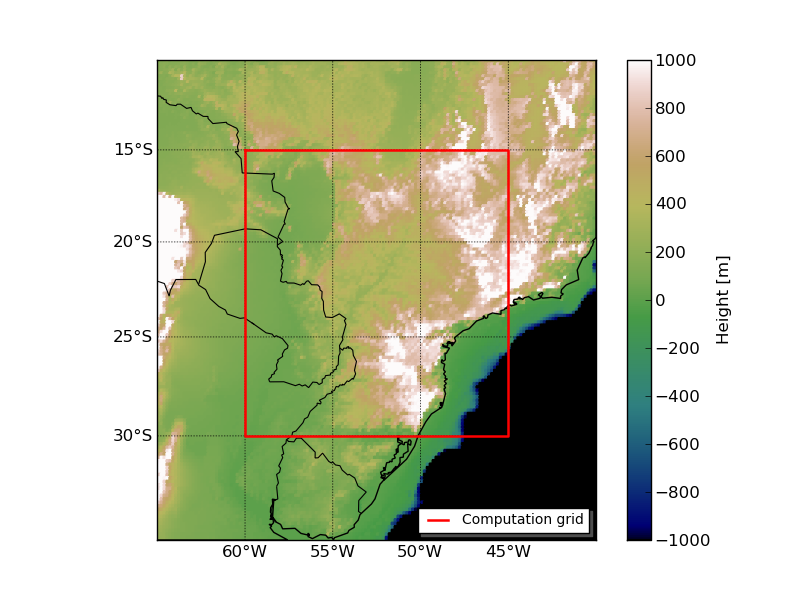
\includegraphics[width=\textwidth]{dem-10min.png}
    \caption{The ETOPO1 10'' DEM of the Paran\'a Basin, southern Brasil.
    \label{fig:dem}}
\end{figure}

\section{Assigning densities}

Program tessmodgen allows us to provide the density value of each tesseroid
through the DEM file. All we have to do is insert an extra column in the DEM
file with the density values of the tesseroids that will be put on each point.
This way we can have the continents with 2.67 $g.cm^{-3}$ and oceans with 1.67 $g.cm^{-3}$.
Notice that the density assigned to the oceans is positive! This is because the
DEM in the oceans will have heights bellow our reference (h=0km) and tessmodgen
will automatically invert the sign of the density values if a point is bellow the reference.
\\
\indent We will use the Python script dem\_density.py to insert the density values into our
DEM and save the result to dem-10min-dens.xyz:

\lstinputlisting[language=sh,firstnumber=3,firstline=3,lastline=4]{run_example.sh}

\hfill\\
\noindent If you don't know Python, you can easily do this step in any other language or
even in Excel. This is what the dem\_density.py script looks like:

\lstinputlisting[language=Python]{dem_density.py}

\hfill\\
The result is a DEM file with a forth column containing the density values
(Figure \ref{fig:dem-dens}):

\lstinputlisting[lastline=10]{dem-10min-dens.xyz}

\begin{figure}[htb]
    \centering
        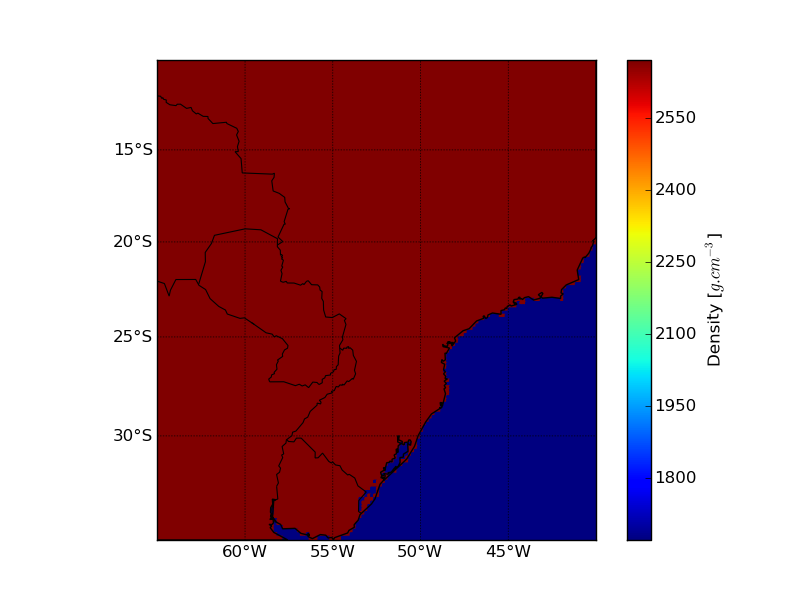
\includegraphics[width=\textwidth]{dem-10min-dens.png}
    \caption{Density values. 2.67 $g.cm^{-3}$ in continents and 1.67 $g.cm^{-3}$
             in the oceans.
    \label{fig:dem-dens}}
\end{figure}

\section{Making the tesseroid model}

Next, we'll use our new file dem-10min-dens.xyz and program tessmodgen to create
a tesseroid model of the DEM:

\lstinputlisting[language=sh,firstnumber=6,firstline=6,lastline=7]{run_example.sh}

\hfill\\
\noindent tessmodgen places a tesseroid on each point of the DEM.
The bottom of the tesseroid is placed on a reference level and the top on the DEM.
If the height of the point is bellow the reference, the top and bottom will be inverted
so that the tesseroid isn't upside-down.
In this case, the density value of the point will also have its sign changed so that you get
the right density values if modeling things like the Moho.
For topographic masses, the reference surface is h=0km (argument -z).
The argument -s is used to specify the grid spacing (10') which will be used to
set the horizontal dimensions of the tesseroid.
Since we didn't pass the -d argument with the density of the tesseroids, tessmodgen
will expect a fourth column in the input with the density values.
\\
\indent The result is a tesseroid model file that should look somthing like this:

\lstinputlisting[lastline=10]{dem-10min-mod.txt}
\hfill\\
\noindent and for the points in the ocean (negative height):

\lstinputlisting[firstnumber=9065,firstline=9065,lastline=9065]{dem-10min-mod.txt}

\section{Calculating the GGT}

Tesseroids now allows use of custom computation grids by reading the computation
points from standard input. This way, if you have a file with lon, lat, and height
coordinates and wish to calculate any gravitational field in those points, all you
have to do is redirect stardard input to that file (using $<$).
All tessg* programs will calculate their respective field, append a column with the result
to the input and print it to stdout.
So you can pass grid files with more than three columns, as long as the first three
correspond to lon, lat and height.
This means that you can pipe the results from one tessg* to the other and have an
output file with many columns, each corresponding to a gravitational field.
The main advantage of this approach is that, in most shell environments, the computation
of pipes is done in parallel. So if your system has more than one core you can get
parallel computation of GGT components with no extra effort.
\\
\indent For convience, we added to the set of tools the program tessgrd to create regular
grids and print them to standard output. So if you don't want to compute on a
custom grid (like us), you can simply pipe the output of tessgrd to the tessg* programs:

\lstinputlisting[language=sh,firstnumber=9,firstline=9,lastline=13]{run_example.sh}

\hfill\\
\noindent The end result of this is file dem-10min-ggt.xyz which will have 9 columns in total.
The first three are the lon, lat and height coordinates generated by tessgrd.
The next six will correspond to each component of the GGT calculated by tessgxx, tessgxy, etc.,
respectively. The resulting GGT is shown in Figure \ref{fig:dem-ggt}.

\lstinputlisting[firstnumber=26,firstline=26,lastline=37]{dem-10min-ggt.xyz}
\hfill\\

\begin{figure}[htb]
    \centering
        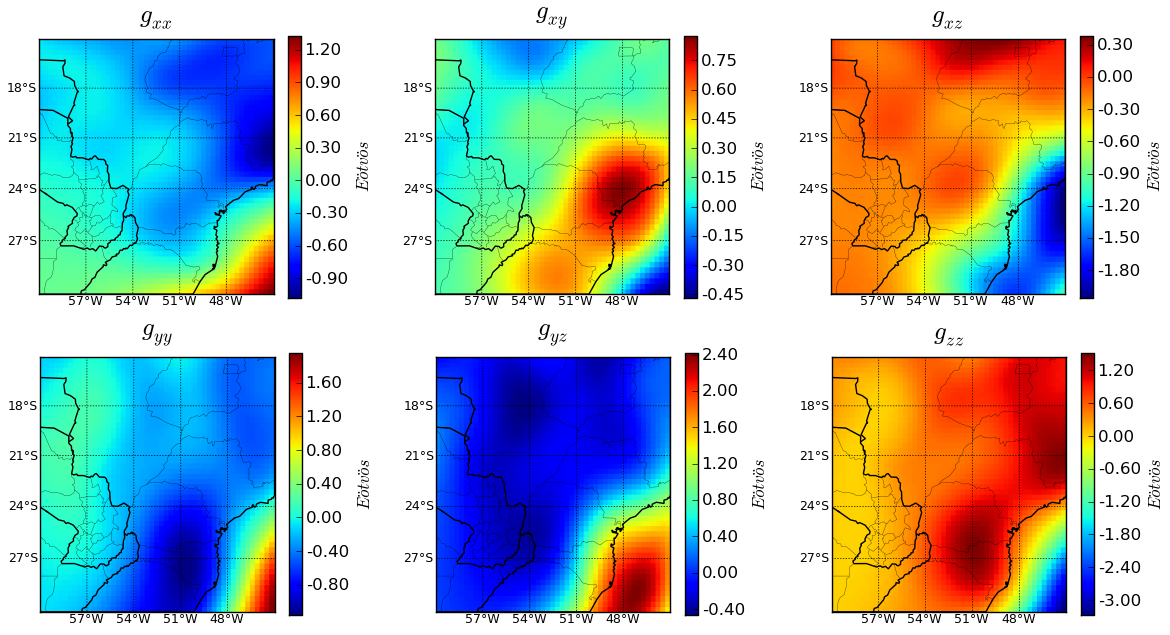
\includegraphics[width=\textwidth]{dem-10min-ggt.png}
    \caption{GGT of caused by the topographic masses.
    \label{fig:dem-ggt}}
\end{figure}

\section{Making the plots}

The plots were generated using the powerfull Python library Matplotlib
(\url{http://matplotlib.sourceforge.net/index.html}).
The script mkplots.py is somewhat more complicated that dem\_density.py and requires
a bit of ``Python Fu''. The examples in the Matplotlib website should give some
insight into how it works.
To hanble the map projections we used the Basemap toolkit of Matplotlib
(\url{http://matplotlib.sourceforge.net/basemap/doc/html/}).

\section{Conclusions}

To wrap up our example, I would like to note that this same processes can be applied
for any sort of interface, like Moho and sediment thickness maps. The difference is
all in the choice of the reference level. For Moho it could be, say, h=-35km.
Another thing to note is that the interface relief should be given as heights.
So sediment thickness would have to be converted into height of the basin's  basement
(which would be negative values).


\end{document}